
%%%%%%%%%%%%%%%%%%%%%%%%%%%%%%%%%%%%%%%%%%%%%%%%%%%%%%%%%%%%%%%%%%%%%%%%%
%           Capítulo 3: Mapeo de Henon
%%%%%%%%%%%%%%%%%%%%%%%%%%%%%%%%%%%%%%%%%%%%%%%%%%%%%%%%%%%%%%%%%%%%%%%%%
\chapter{Ejemplos de aplicación del método}
\section{Mapeo Estándar}
En el capítulo anterior ya mostramos cómo se aplica el método de manera algebráica para el caso de este mapeo. Utilizando el método ya programado se hicieron diferentes cálculos para comparar con los resultados presentados en \citep{Mireles} . Una de las razones de estudiar el mapeo estándar, además de usarlo como una forma de validación, es porque del mapeo conocemos muchas cosas. Por otro lado queremos mostrar lo importante que es tener una parametrización analítica. Aunque el estudio cualitativo del mapeo puede darnos información útil, tener una parametrización de las variedades relacionadas a sus puntos fijos convierte el análisis en algo cuantitativo y semi-analítico. El objetivo de esta sección es mostrar algunas de las cosas que son posibles alcanzar en términos de este análisis, además de la forma en la que se usa el método desde Julia.\\

En el mapeo estándar \ref{mapeo estandar} uno de los puntos fijos es el origen de coordenadas $x_{1}=(0,0)$. Utilizando el método programado se calcularon las variedades estables e inestables para diferentes valores del parámetro en el mapeo. El objetivo de hacer éstas fue reproducir los resultados de J.D. Mireles que presenta en sus notas \cite{Mireles}. En tales notas no aparece el orden del polinomio ni el error específico, sin embargo se intentó reproducir al menos gráficamente los resultados. Dependiendo del orden del polinomio que se calcule y del parámetro del mapeo se podrá llegar más lejos del punto fijo.  
\begin{figure}[H]
 \centering
 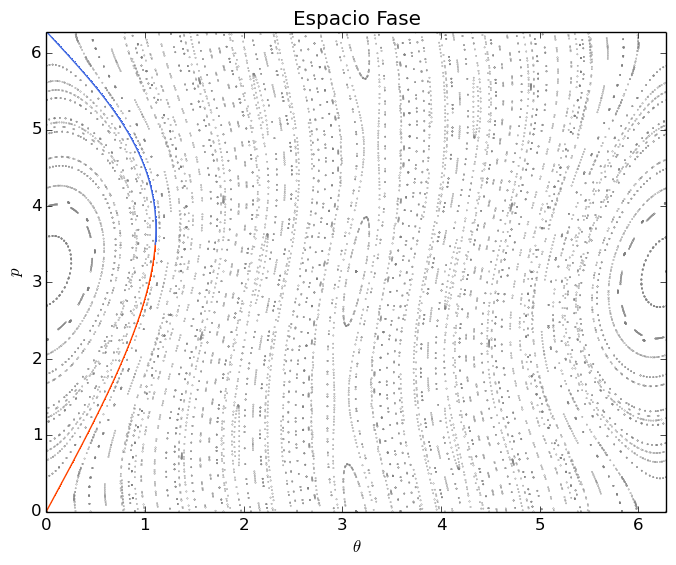
\includegraphics[scale=0.6]{estandark03}
 \caption{$W^{s},W^{u}$ de orden 25 en el mapeo estándar con $\kappa=0.3$ y $t_{max}=3.$}
 \label{estandar03}
\end{figure}

\begin{figure}[H]
\centering
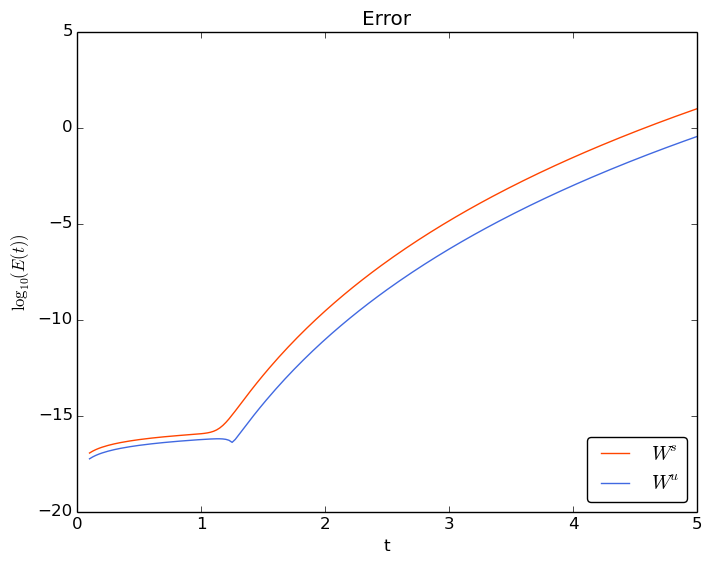
\includegraphics[scale=0.6]{error_est_k03} 
\caption{Error en las variedades de orden 25 ,$\kappa=0.3$}
\label{error est k03}
\end{figure}



\begin{figure}[H]
\centering
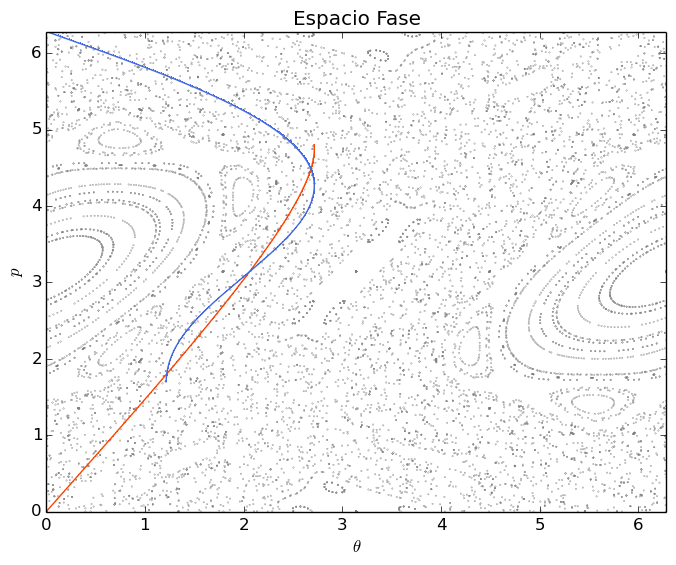
\includegraphics[scale=0.6]{estandark15}
\caption{$W^{s},W^{u}$ de orden 80 en el mapeo estándar con $\kappa=1.5$}
\label{estandar15}
\end{figure}

\begin{figure}[H]
\centering
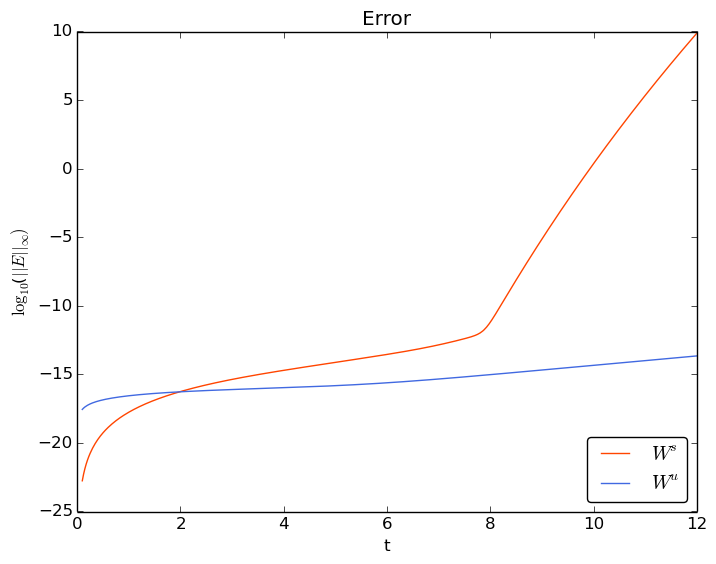
\includegraphics[scale=0.6]{error_est_k15} 
\caption{Error en las variedades de orden 80 , $\kappa=1.5$}
\label{error est k15}
\end{figure}




\begin{figure}[H]
\centering
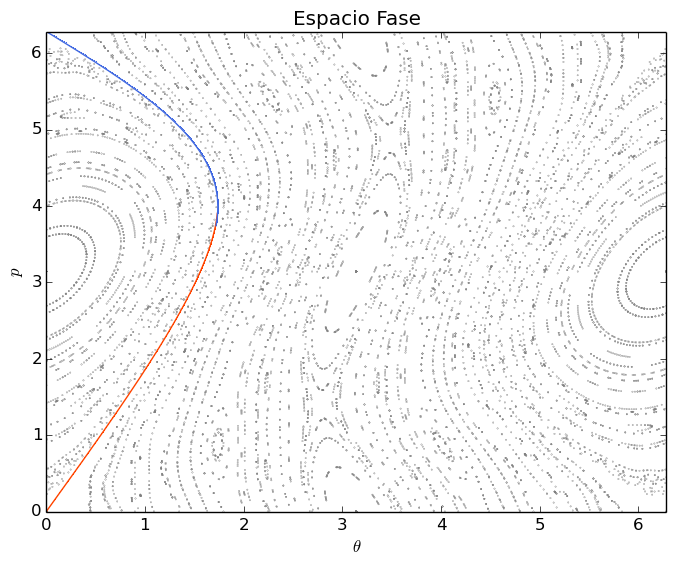
\includegraphics[scale=0.6]{estandark07}
\caption{$W^{s},W^{u}$ de orden 70 en el mapeo estándar con $\kappa=0.7$}
\label{estandar07}
\end{figure}

\begin{figure}[H]
\centering
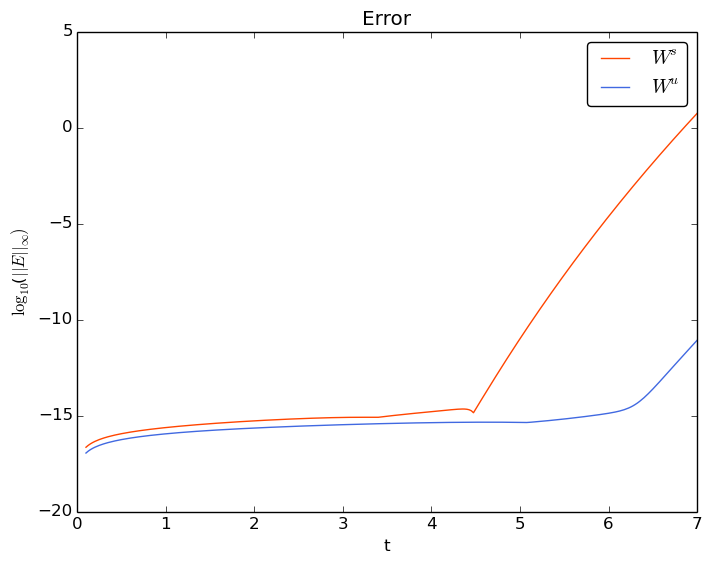
\includegraphics[scale=0.6]{error_est_k07} 
\caption{Error en las variedades , $\kappa=0.7$}
\label{error est k07}
\end{figure}


En las figuras \ref{estandar03}-\ref{error est k07} se muestran los resultados de la parametrización de las variedades estable e inestable asociadas al punto fijo $\mathbf{x}=(0,0)$ para diferentes valores del parámetro $\kappa$, junto con cada una aparece su respectiva gráfica del error numérico.  Los cálculos se hicieron utilizando números de punto flotante de 64 bits(Float64). Para las figuras \ref{estandar03}, \ref{estandar07} se puede ver que las variedades se juntan de manera que parecen ser tangentes, mientras que para el caso de la figura \ref{estandar15} observamos varias intersecciones entre las variedades. En todos los casos el error se comporta de manera similar, manteniendose prácticamente constante hasta cierto valor del parámetro $t$ y creciendo de forma exponencial después del mismo. La curva será entonces confiable hasta valores del parámetro que no excedan el punto donde el error crece rápidamente.  \\


Para observar como cambiaba el comportamiento del error respecto del orden de la parametrización se calcularon polinomios de diferente orden que parametrizan a la variedad inestable del mapeo con $\kappa=0.3$,el resultado se muestra en la figura \ref{erroresf64}. Observamos que mientras más grande sea el orden del polinomio mejor es la aproximación, pues podemos llegar a valores del parámetro más grandes, que se traduce en ir más lejos en la variedad inestable. \\

\begin{figure}[H]
\centering
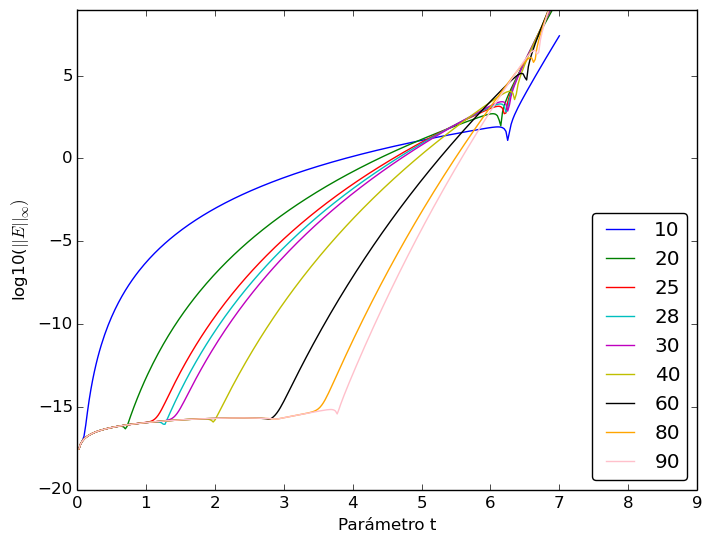
\includegraphics[scale=0.6]{error_estandar_orden}
\caption{Curvas de error para diferentes órdenes en el mapeo estándar,$\kappa=0.3$ }
\label{erroresf64}
\end{figure}
A fin de mostrar que el error es de alguna manera controlable se usaron números de presición extendida para hacer cálculos análogos a los anteriores. En la figura \ref{erroresBig} se muestran los resultados para parametrizaciones de ordenes entre $10$ y $80$. Observamos un comportamiento análogo, de tal manera que para cada orden diferente de parametrización hay un valor diferente del parámetro en el cuaĺ pasa de un error que no crece significativamente a un error que crece de manera abrupta. También notamos que al usar presición extendida el error cerca del punto fijo es imperceptible pero en la parte donde crece, tiene un crecimiento más pronunciado que en el caso de números de punto flotante. 

\begin{figure}[H]
\centering
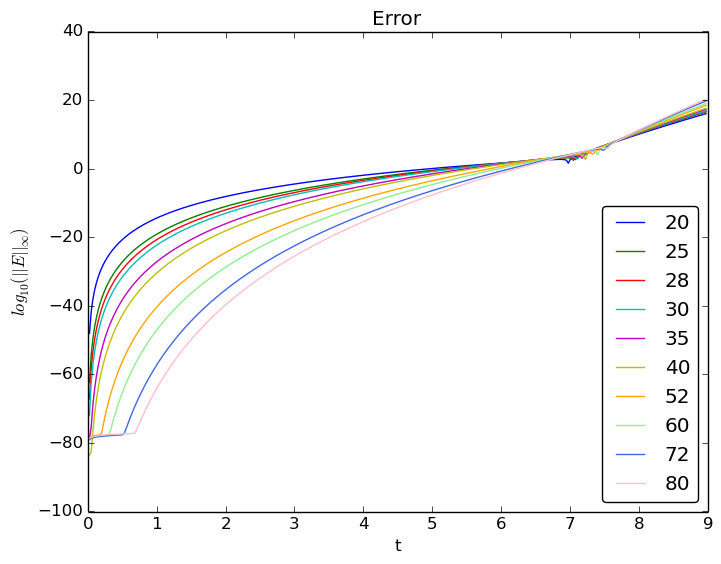
\includegraphics[scale=0.6]{error_estandar_orden_big}
\caption{Curvas de error para diferentes órdenes usando precisión extendida ,$\kappa=0.3$ }
\label{erroresBig}
\end{figure}

Como ya mencionamos antes la variedad inestable del mapeo inverso corresponde a la variedad estable del mapeo, por lo que si se usa el mismo método calculando la variedad inestable del mapeo inverso \ref{mapeo estandar inverso} podemos controlar mejor el error numérico. Para mostrar esto hicimos una comparación parametrizando la variedad estable mediante el mapeo inverso y el mapeo inicial. Los polinomios fueron del mismo orden y lo que se observó en el error se muestra en la figura \ref{erroresinverso}.
\begin{eqnarray}
f_{k}^{-1}(\theta,p) = \left[\begin{array}{c}
\theta  -k\sin(p-\theta) \\
p -\theta
\end{array}\right] mod(2\pi) \label{mapeo estandar inverso}
\end{eqnarray}

\begin{figure}[H]
\centering
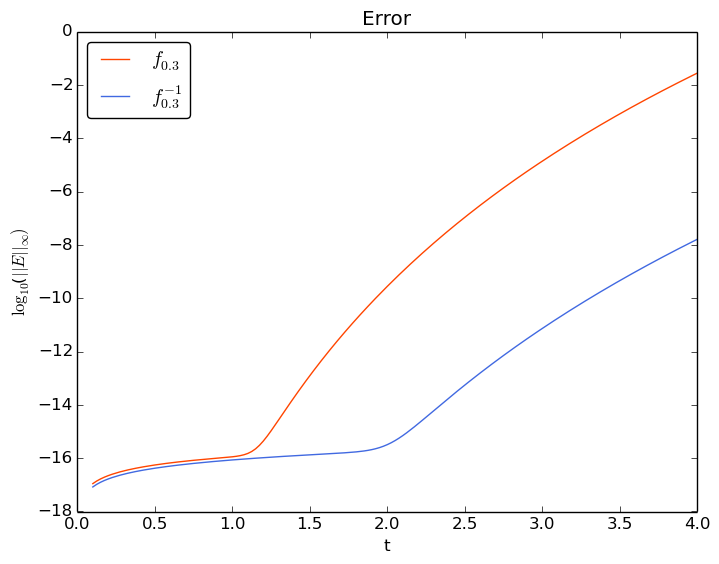
\includegraphics[scale=0.6]{mapeoinver}
\caption{Error para las parametrizaciones usando el mapeo y el mapeo inverso ,$\kappa=0.3, orden=20$ }
\label{erroresinverso}
\end{figure}




\section{Mapeo de Hénon}
El mapeo de Hénon se define como \cite{devaney}
\begin{eqnarray}
\mathbf{f}_{a,b}(x,y)=\left( \begin{array}{lcc}
             a-by-x^{2}\\
             \\ x
             \end{array}
             \right) \label{Henon}
\end{eqnarray}

siendo el mapeo inverso
\begin{eqnarray}
\mathbf{f}^{-1}_{a,b}(x,y)=\left( \begin{array}{lcc}
             y\\
             \\ (x+y^{2}-a)/-b
             \end{array}.
             \right) \label{HenonI}
\end{eqnarray} 

       
Para poder analizarlo debemos linearizar el sistema. Primero obtenemos el jacobiano 
            
\begin{eqnarray}
D\mathbf{f}_{a,b}(x,y)= \left( \begin{array}{lcc}
                -2x & -b\\
                \\ 1 & 0
                \end{array}
                \right)
\end{eqnarray}

                
Notamos que el determinante del jacobiano no es igual a uno sino $\det(D\mathbf{f}_{a,b}(x,y))=b$.
El determinante es constante, entonces será hamiltoniano en el caso en que $b$ sea igual a uno o menos uno. Analizaremos estos casos, primero encontrando los puntos fijos
\begin{eqnarray}
\mathbf{f}_{a,b}(x,y)=\left( \begin{array}{lcc}
               a-by-x^{2}\\
               \\ x
               \end{array}
               \right) = \left(\begin{array}{lc}
               x \\
               \\ y
               \end{array}
               \right)
\end{eqnarray}
              
lo que implica que $a-by-x^{2}=x$ y $x=y$ de donde es claro que la primer ecuación queda
\begin{eqnarray*}
x^{2}+(b+1)x-a=0
\end{eqnarray*}
que se puede resolver usando la fórmula general
\begin{eqnarray*}
x=\frac{-(b+1)\pm ((b+1)^{2}+4a)^{1/2} }{2}
\end{eqnarray*}
para el caso en que $b=1$ se tiene
\begin{eqnarray}
x=\frac{-2\pm 2(1+a)^{1/2} }{2}
\end{eqnarray}
Al escoger $b=1$ garantizamos estar en un sistema hamiltoniano, mientras que $a$ debe escogerse de manera que resulten puntos fijos hiperbólicos. La figura \ref{Henon1} muestra un ejemplo en cálculos de variedades para el mapeo de Hénon, junto con el error. 
\begin{figure}[H]
\centering
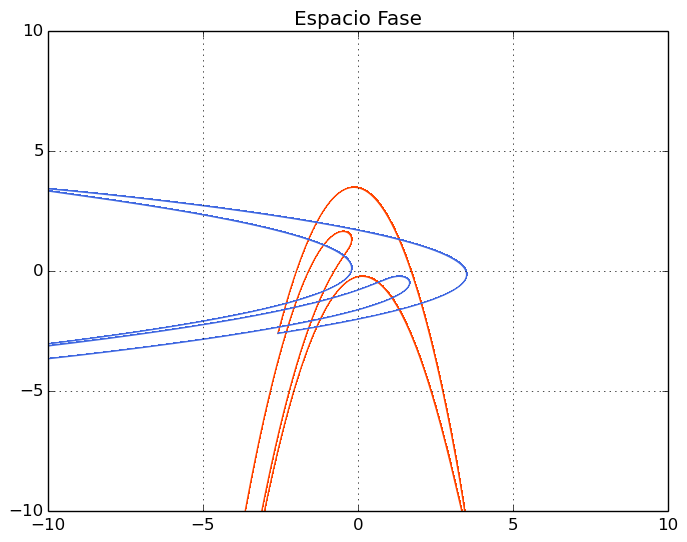
\includegraphics[scale=0.6]{henon1}
\caption{$W^{u}$ de orden 336 y $t_{max}=43534$ ,$W^{s}$ de orden 7363 y $t_{max}=87643$ para el mapeo de Hénon con a=1.5,b=1}
\label{Henon1}
\end{figure}

\begin{figure}[H]
\centering
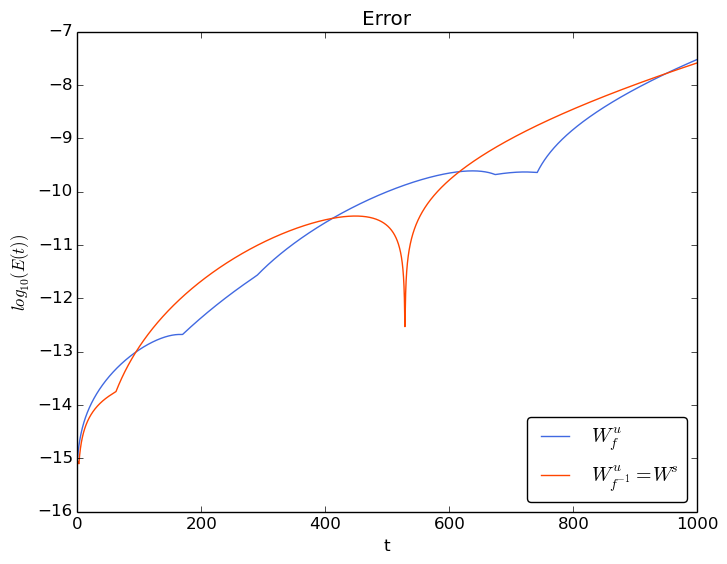
\includegraphics[scale=0.6]{ErrorHenon1}
\caption{Error en el mapeo de Hénon asociado a las variedades de la figura \ref{Henon1}.}
\label{ErrorHenon1}
\end{figure}
Las variedades que aparecen en la figura \ref{Henon1} fueron calculadas con el mapeo de Hénon inicial \ref{Henon}, las variedades se observan simétricas, aún así las parametrizaciones son diferentes. Puede verse en el error, figura \ref{ErrorHenon1}, que la variedad estable tiene un mayor error que la variedad inestable, mientras en la inestable el error cambia cinco órdenes de magnitud, en todo el intervalo del parámetro, el error de la variedad estable cambia en al menos quince órdenes de magnitud. \\

A diferencia del mapeo estándar en éste mapeo las órbitas pueden irse al infinito, es decir no están  constreñidas en una sección fija, lo que representa un mayor reto en cuanto a la parametrización ya que el polinomio debe ser tal que pueda regresar varias veces. De hecho podemos observar que se necesitan valores realmente grandes, comparados con los del mapeo estándar, para observar los cruces de las variedades. También esta situación hace que el error numérico sea mayor que para el estándar. \\

En las figuras \ref{Henon2}, \ref{Henon3} se muestran las variedades calculadas de la misma manera en la que se calcularon para la figura \ref{Henon1}. En \ref{Henon2} las curvas son más cerradas y se necesita de un polinomio de orden mayor que en el caso de \ref{Henon3} para observar los cortes. 
\begin{figure}[H]
\centering
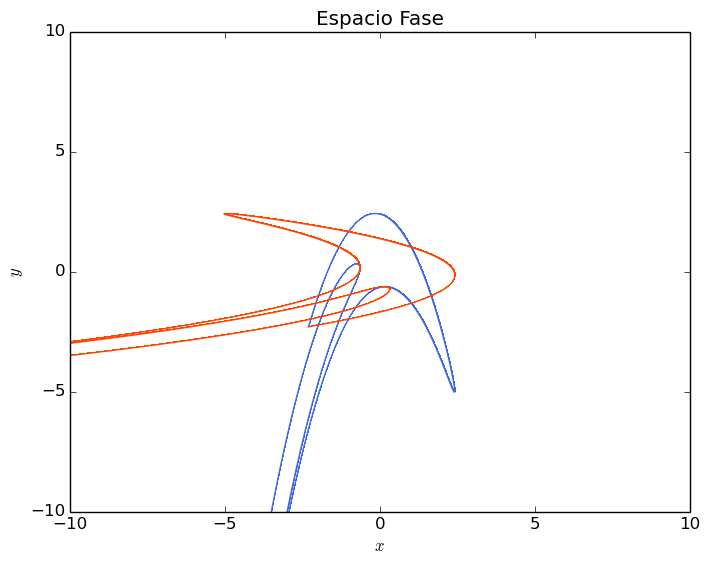
\includegraphics[scale=0.6]{henon2}
\caption{$W^{u}$ de orden 98339 y $t_{max}=664564$, $W^{s}$ de orden 6464 y $t_{max}=87t6423$ para el mapeo de Hénon con a=0.7,b=1.}
\label{Henon2}
\end{figure}


\begin{figure}[H]
\centering
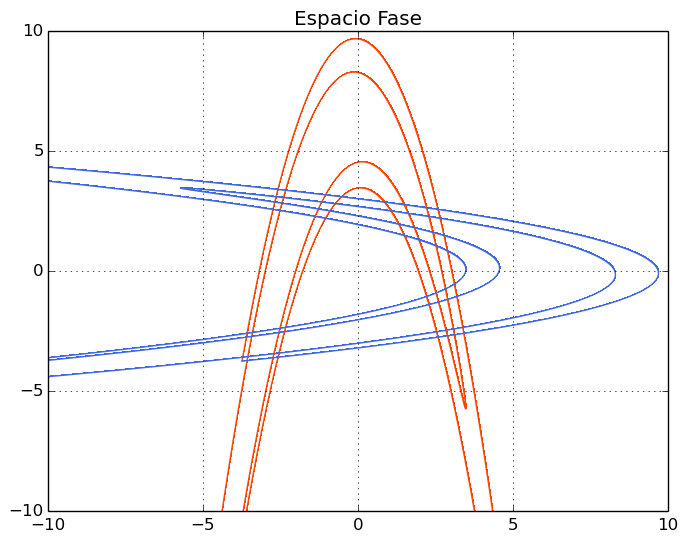
\includegraphics[scale=0.6]{henon3}
\caption{$W^{u}$ de orden 874873 y $t_{max}=7yt4$,$W^{s}$ de orden 2321 y $t_{max}=8764$ para el mapeo de Hénon con a=6.5,b=1.}
\label{Henon3}
\end{figure}

Asi que con el orden suficiente es posible observar los cruces de ambas variedades, retomaremos esto en la última sección. 

\section{Mapeo exponencial}
El último mapeo que se estudió fue uno presentado en el artículo \citep{Jung} el cual queda definido por 
\begin{eqnarray}
\mathbf{j}_{a}(x,y)=\left(\begin{array}{lcc}
             x+y\\
             \\ y+af(x+y)
             \end{array}\right)
\label{Jung}
\end{eqnarray}

que describe el movimiento de una partícula pateada , donde la coordenada $x$ representa la posición en una dimensión mientras que la coordenada $y$ es el momento, $a$ es un parámetro libre. La función $f$ es la responsable de describir la fuerza aplicada, en el artículo \cite{Jung} se escoge
\begin{eqnarray*}
f(x)=x(x-1)e^{-x}.
\end{eqnarray*}
Al cual le corresponde su inverso
\begin{eqnarray}
\mathbf{j}^{-1}_{a}(x,y)=\left(\begin{array}{lcc}
             x-y+ax(x-1)e^{-x}\\
             \\ y-ax(x-1)e^{-x}
             \end{array}\right).
             \label{jungI}
\end{eqnarray}
En este sistema los puntos fijos encontrados son $x_{0}=(1,0),x_{1}=(0,0)$ donde $x_{0}$ es un punto fijo hiperbólico. El punto $x_{1}$ es un punto elíptico mientras el valor del parámetro sea menor a 4, para valores de $a \geq 4$ se torna inverso hiperbólico.\\

Aplicando el mismo mecanismo que en los casos pasados se obtuvieron las figuras \ref{jung1}-\ref{errorjung2} que muestran cómo se comportan las variedades aún en el caso en que el sistema no sea completamente hiperbólico. Como en los casos anteriores el error asociado a la variedad estable es mayor que el asociado a la inestable. Al parecer la forma exponencial del mapeo también hace que el error crezca de manera exponencial para la estable. El orden al que se debe llegar en los polinomios para observar algunos de los cortes de las variedades es más alto en comparación con el mapeo de Hénon debido a que en este caso se esta aproximando una función exponencial.

\begin{figure}[H]
\centering
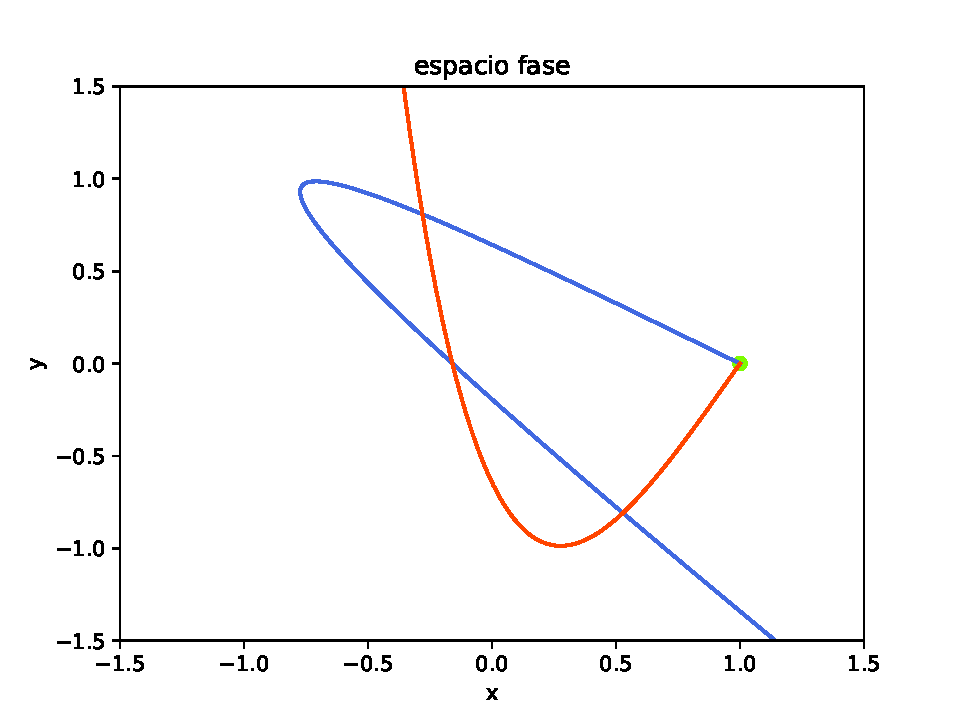
\includegraphics[scale=0.6]{jung34}
\caption{$W^{s}$ de orden 54848 con $t_{max}=7474$ , $W^{u}$ de orden 234 con $t_{max}=7484$, con $a=3.4$ en el punt fijo $x_{0}$}
\label{jung1}
\end{figure}


\begin{figure}[H]
\centering
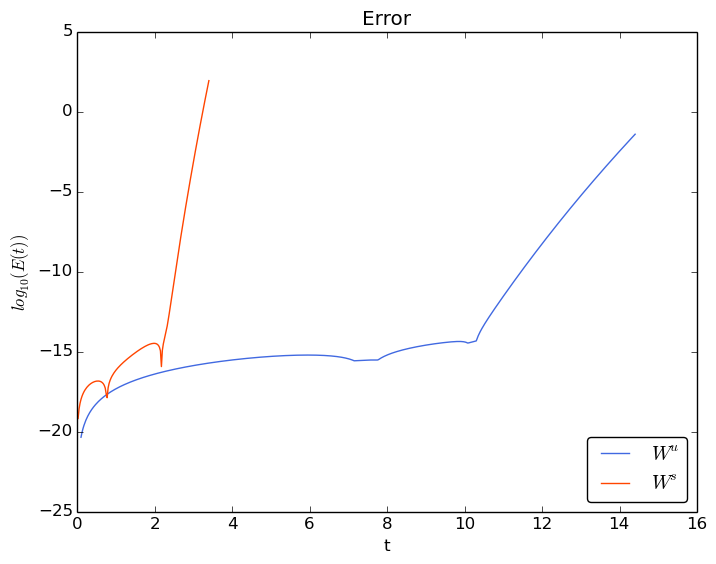
\includegraphics[scale=0.6]{error_jung34}
\caption{Error asociado a $W^{s},W^{u}$ con $a=3.4$}
\label{errorjung1}
\end{figure}




\begin{figure}[H]
\centering
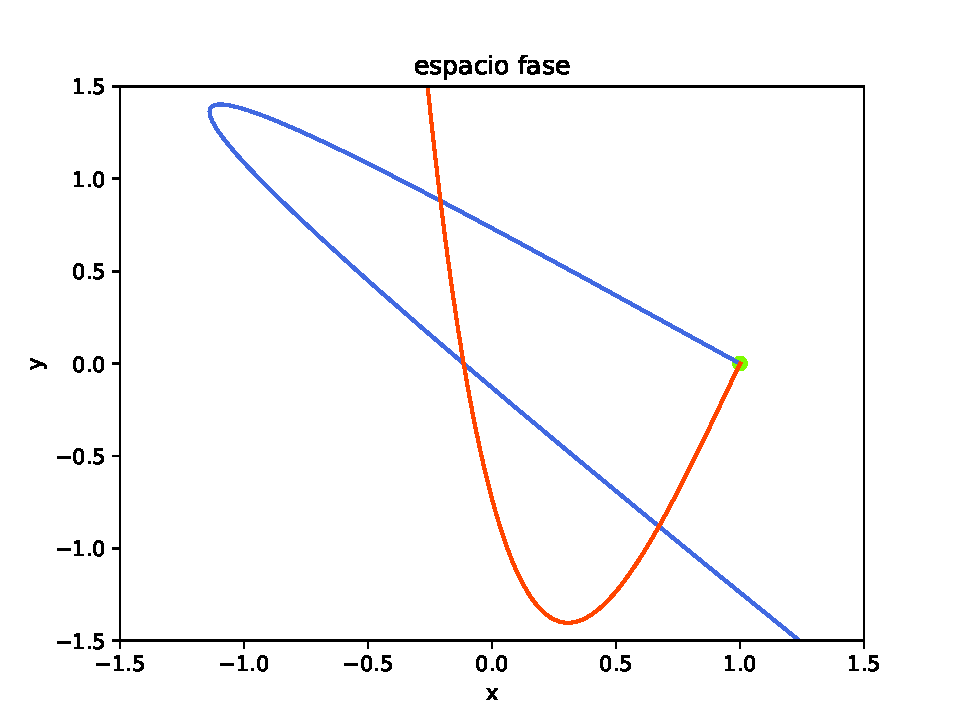
\includegraphics[scale=0.6]{jung57}
\caption{$W^{s}$ de orden 54848 con $t_{max}=7474$ , $W^{u}$ de orden 234 con $t_{max}=7484$, con $a=5.7$ en el punto fijo $x_{0}$}
\label{jung2}
\end{figure}


\begin{figure}[H]
\centering
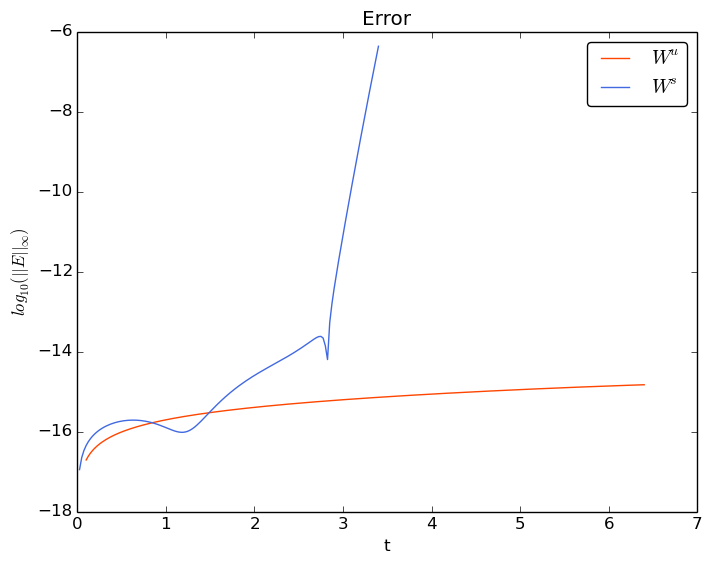
\includegraphics[scale=0.6]{error_jung57}
\caption{Error asociado a $W^{s},W^{u}$ con $a=5.7$ en $x_{0}$}
\label{errorjung2}
\end{figure}


\section{Convergencia}
Además de medir el error asociado a la parametrización consideramos importante tomar en cuenta la convergencia de los coeficientes de los polinomios. En casos como el mapeo exponencial en que las variedades se acercan a puntos fijos de diferente naturaleza puede ocurrir que tal cercanía afecte la forma de parametrización. Para ello se implementaron dos formas de revisar la convergencia, la de Hadamard \ref{hadamard} y la de tres términos \ref{tres terminos}. \\

La figura \ref{convergenciaEst15} muestra la convergencia de los polinomios de orden 25 que parametrizan la variable $\theta$ en el mapeo estádar para las variedades estable e inestable con $\kappa=1.5$ a la que correponde el espacio fase mostrado en \ref{estandar15}. En el caso de la variedad estable se ve que los coeficientes cambian de manera abrupta al principio pero después de cierta $n$ el cociente es casi cero. Para el caso de la variedad inestable los coeficientes cambian de manera suave y el cociente también se acerca a cero. En ambos casos podemos decir que los coeficientes de la parametrización convergen a cero.  
\begin{figure}[H]
\centering
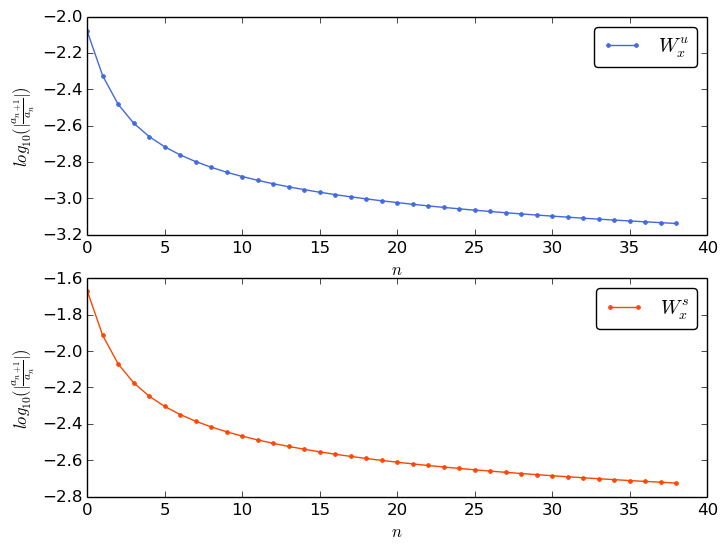
\includegraphics[scale=0.6]{converEst15}
\caption{Convergencia de Hadamard asociada a los polinomios para $\theta$ en las variedades del mapeo estándar con $\kappa=1.5$}
\label{convergenciaEst15}
\end{figure}

La figura \ref{convergenciaHenon1} muestra la convergencia de las parametrizaciones de orden 45 para la variable $x$ en el mapeo de Hénon con $a=1.5$. En ambos casos la convergencia parece suave y tiende a cero y igual que en el caso del mapeo estándar.

\begin{figure}[H]
\centering
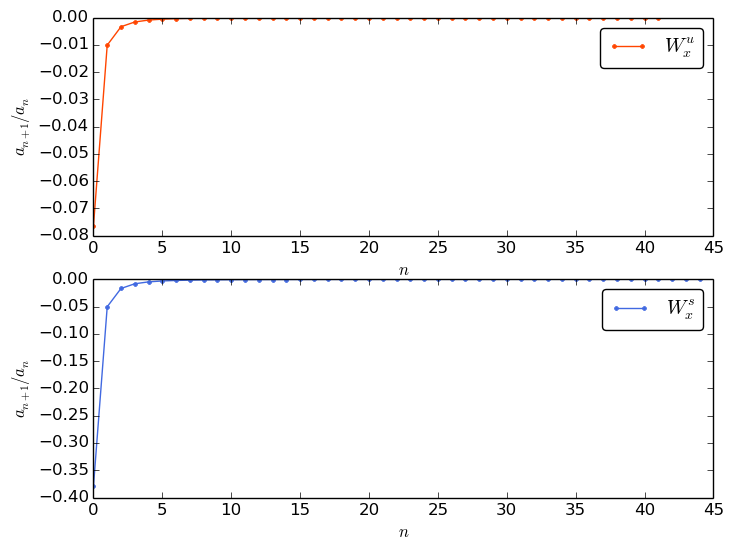
\includegraphics[scale=0.6]{converHenon1}
\caption{Convergencia de Hadamard asociada a los polinomios para $x$ en las variedades del mapeo de Hénon con $a=1.5$}
\label{convergenciaHenon1}
\end{figure}


Para el mapeo exponencial realizamos los dos criterios de convergencia. La figura \ref{convergenciaJH} muestra el criterio de Hadamard \ref{hadamard} y se ve que el cociente de los coeficientes tiende a cero. En la figura \ref{convergenciaJ3} se usó el criterio de tres términos \ref{tres terminos} y se observa el mismo comportamiento. 

\begin{figure}[H]
\centering
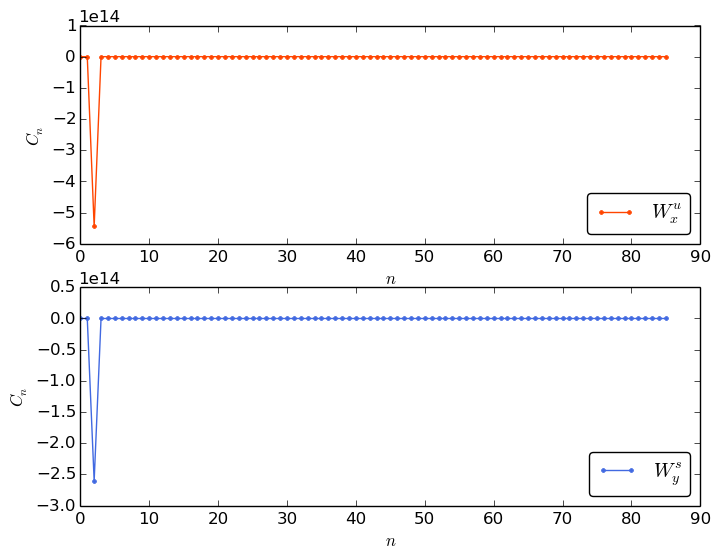
\includegraphics[scale=0.5]{convergenciaJungH}
\caption{Convergencia de Hadamard asociada a los polinomios de orden $87$ para $x$ en las variedades del mapeo exponencial con $a=5.7$.}
\label{convergenciaJH}
\end{figure}


\begin{figure}[H]
\centering
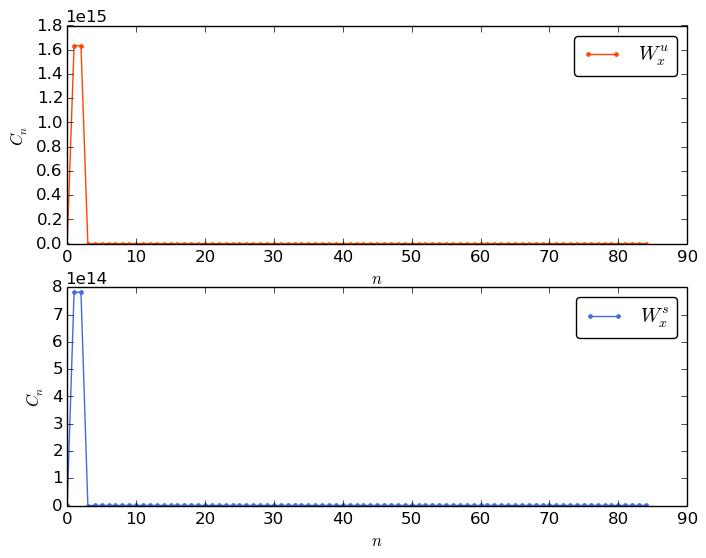
\includegraphics[scale=0.5]{convergenciaJungT}
\caption{Convergencia de tres términos asociada a los polinomios de orden $87$ para $x$ en las variedades del mapeo exponencial para $a=5.7$.}
\label{convergenciaJ3}
\end{figure}



\section{Existencia de puntos homoclínicos}
\subsection{Estándar}
Siendo que el resultado son polinomios se puede aplicar el método de Newton en dos dimensiones o cualquier otro para resolver $P^{u}=P^{s}$. Por surte existe un paquete en IJulia que hace aritmética de intervalos \texttt{ValidatedNumerics} \ref{interval} , dentro de este se encuentra el paquete que calcula raíces de funciones en términos de intervalos. En forma simple si $[a,b],[c,d]$ son intervalos en $\mathbb{R}$ entonces es posible definir las operaciones básicas, por ejemplo la suma $+$
\begin{eqnarray}
[a,b]+[c,d]=[a+b,c+d]
\end{eqnarray}
resulta bastante simple e intuitiva; la definición de otras operaciones puede verse en \ref{ramon}. La finalidad en nuestro caso de usar intervalos $[a,b]$ en lugar de un valor $x$ es que al encontrar un intervalo podemos afirmar que en tal se encuentra la raíz, sin embargo al calcular la raíz como un valor debemos tomar en cuenta que puede que ese valor no sea el exacto. Es decir debido a procesos de redondeo, así como de errores en la interpretación de un número real de manera computacional puede que nuestro valor de la raíz calculado de manera convencional no sea el valor correcto. Sin embargo al hacer aritmética de intervalos no encontramos la raíz en sí , encontramos un intervalo en donde podemos garantizar que se encuentra la raíz verdadera. Los métodos usados para calcular raíces con intervalos se valen de la generalización del método de Newton.

Para nuestro caso resulta que el programa arroja dos polinomios asociados a cada variedad, si definimos 
\begin{eqnarray}
P:=P^{u}(t)-P^{s}(t')=0
\label{CorteV}
\end{eqnarray}
podemos encontrar las intersecciones en un intervalo de 2 dimensiones que será $[a,b]\times[c,d]$ con $a,b,c,d \in \mathbb{R}$. Usando esto en el mapeo stándar con una tolerancia de $10^{-5}$ se encontraron la siguientes intersecciones para un caso específico.
\begin{figure}[H]
\centering
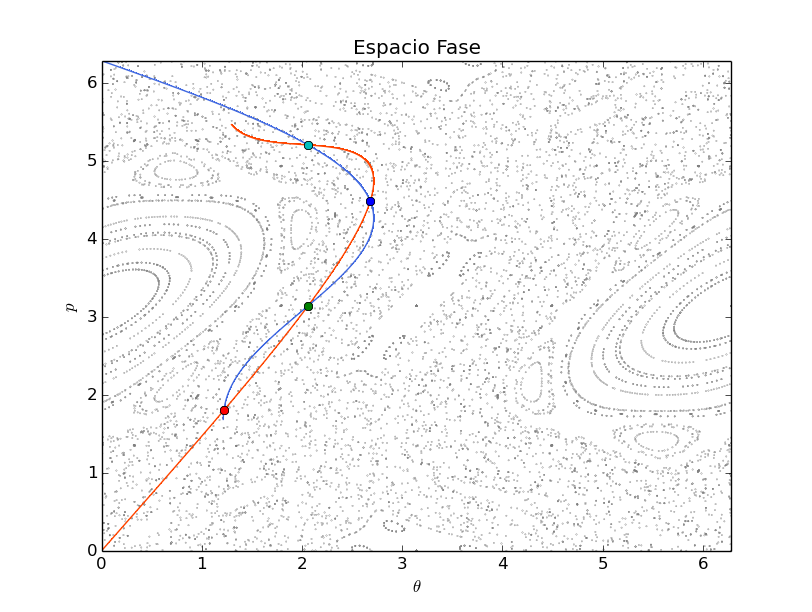
\includegraphics[scale=0.4]{cruce_estandar}
\caption{Cruces de $W^{u},W^{s}$ para el mapeo estándar con $k=1.5$ }
\label{cruce_estandar}
\end{figure}







\subsection{Hénon}
Como mencionamos en el mapeo estándar usando el paquete de aritmética de intervalos se pueden calcular las intersecciones de las variedades estable e inestable. En este caso para el mapeo de Hénon, donde el parámetro $a=1.5$ con un polinomio de orden 45, se usó el método con una tolerancia de $10^{-6}$ además de usar el mapeo inverso \ref{HenonI}, para calcular la variedad estable. 
 
Lo que resultó de resolver \ref{CorteV} fueron los siguientes intervalos:
\begin{itemize}
\item[a)] Root$([-1.36597, -1.36596] \times [166.749, 166.75]$, :unique)
\item[b)] Root$([-5.26555, -5.26554] \times [129.577, 129.578]$, :unique)
\item[c)] Root$([-6.77613, -6.77612] \times [33.6142, 33.6143]$, :unique)
\item[d)] Root$([-5.54438e-07, 0] \times [0, 5.54438e-07]$, :unknown)     
\item[e)] Root$([-26.1208, -26.1207] \times [26.1207, 26.1208]$, :unique)  
\item[f)] Root$([-33.6143, -33.6142] \times [6.77612, 6.77613]$, :unique)  
\item[g)] Root$([-129.578, -129.577] \times [5.26554, 5.26555]$, :unique) 
\item[h)] Root$([-166.75, -166.749] \times [1.36596, 1.36597]4$, :unique)
\end{itemize}

La leyenda \texttt{unique} concluye que hay una raíz en el intervalo y es única, mientras que \texttt{unknown} nos dice que no puede concliur si hay una o más. Si notamos el tercer intervalo contiene al cero $(t,t')=(0,0)$ en el cual se cortan las variedades pues representa el punto fijo. Para los intervalos encontrados se hizo una gráfica que representa el intervalo donde se encuentra el cruce. 


\begin{figure}[H]
\centering
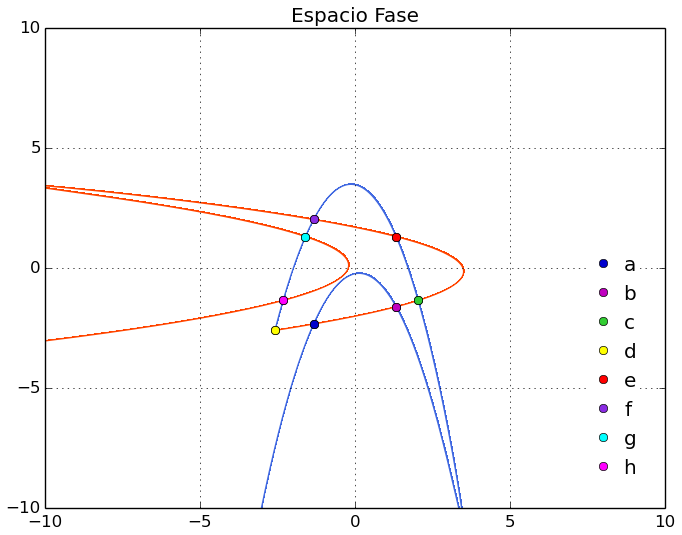
\includegraphics[scale=0.5]{crucesL}
\caption{Cruces de $W^{u},W^{s}$ encontrados en el intervalo $[-400.,0.] \times [0.,400.]$ }
\label{cruces}
\end{figure}

Donde cada punto indica un cruce econtrado, el punto de color es sólo para indicar cuaĺes fueron encontradas. En cuanto a el intervalo real en donde se encontró la intersección podemos encontrar las siguientes gráficas.


\begin{figure}[H]
\centering
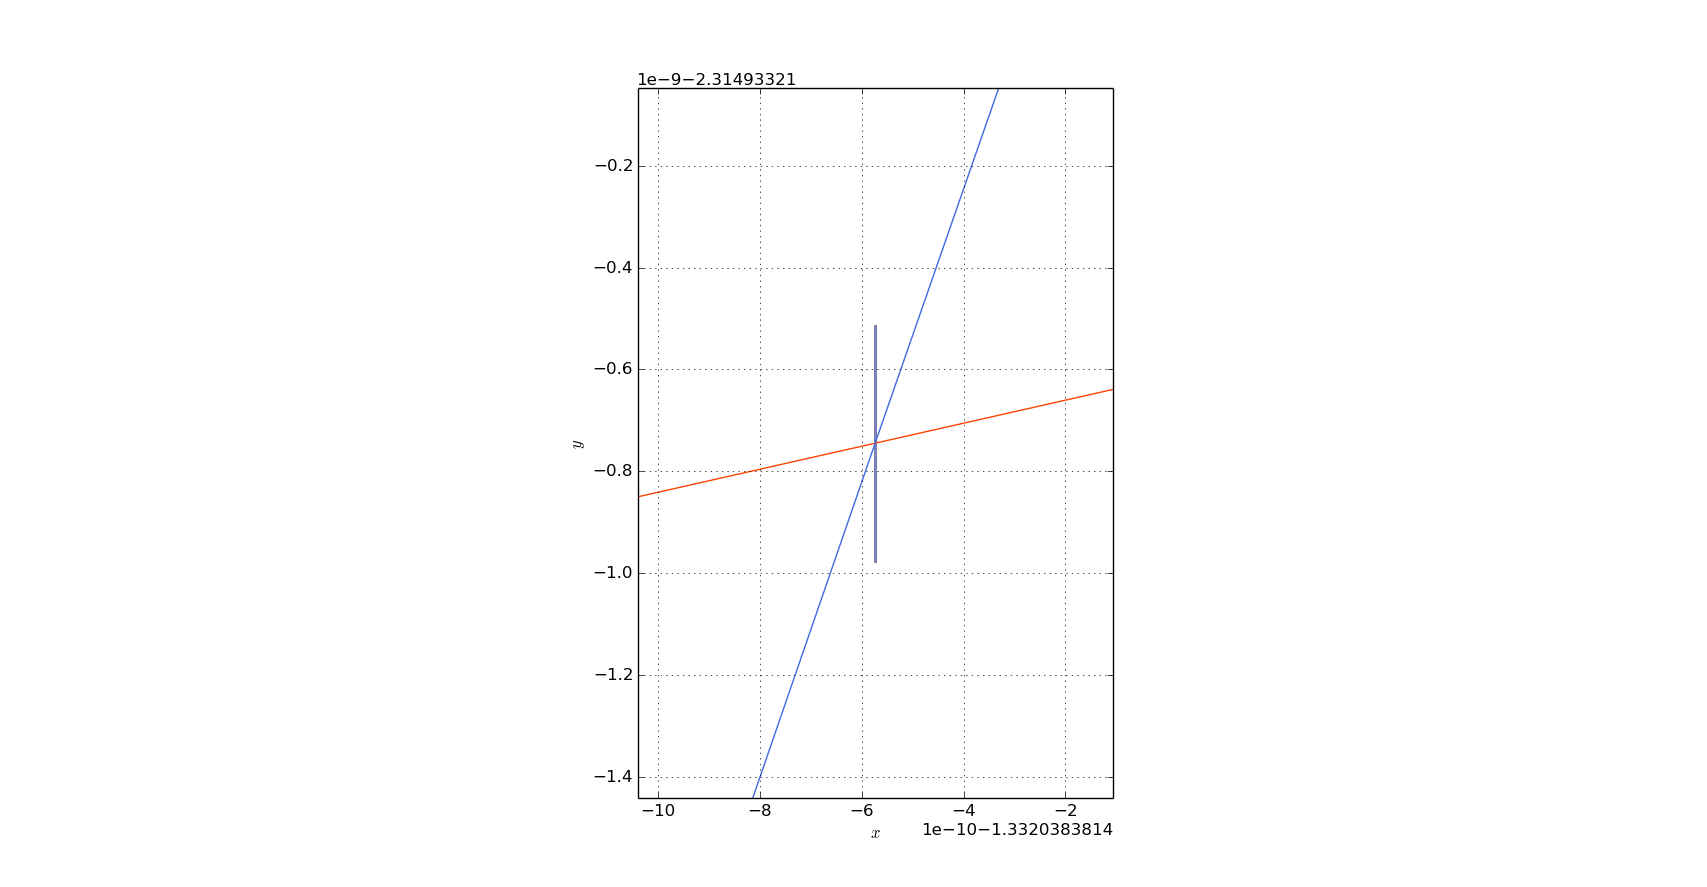
\includegraphics[scale=0.4]{cruce1}
\caption{Cruce de $W^{u},W^{s}$ encontrado con el intervalo a}
\label{cruce1}
\end{figure}

\begin{figure}[H]
\centering
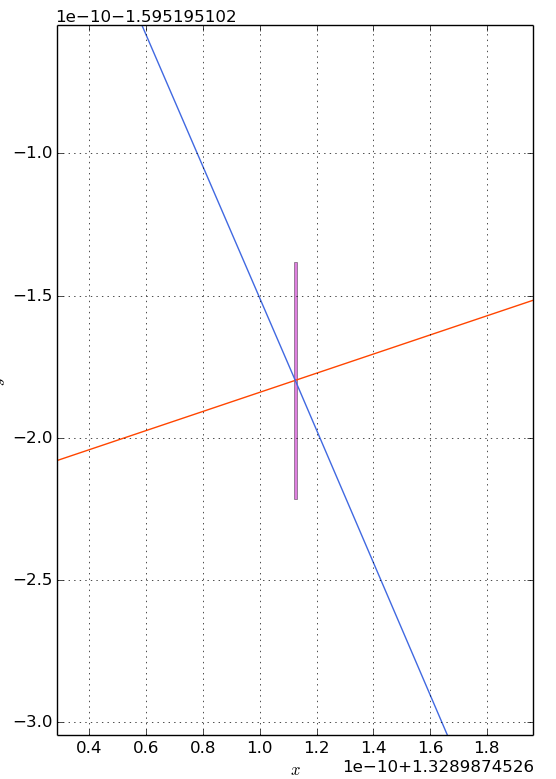
\includegraphics[scale=0.4]{cruce2}
\caption{Cruce de $W^{u},W^{s}$ encontrado con el intervalo b}
\label{cruce2}
\end{figure}


\begin{figure}[H]
\centering
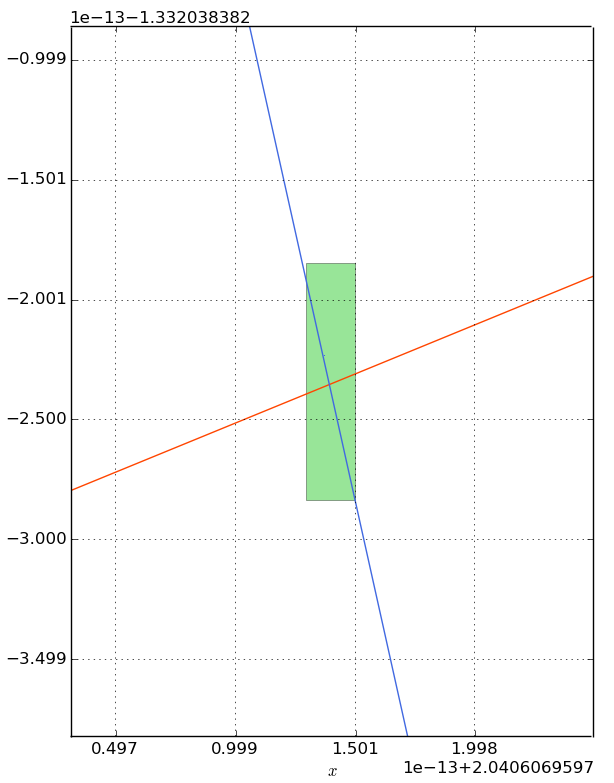
\includegraphics[scale=0.4]{cruce3}
\caption{Cruce de $W^{u},W^{s}$ encontrado con el intervalo c }
\label{cruce3}
\end{figure}


\begin{figure}[H]
\centering
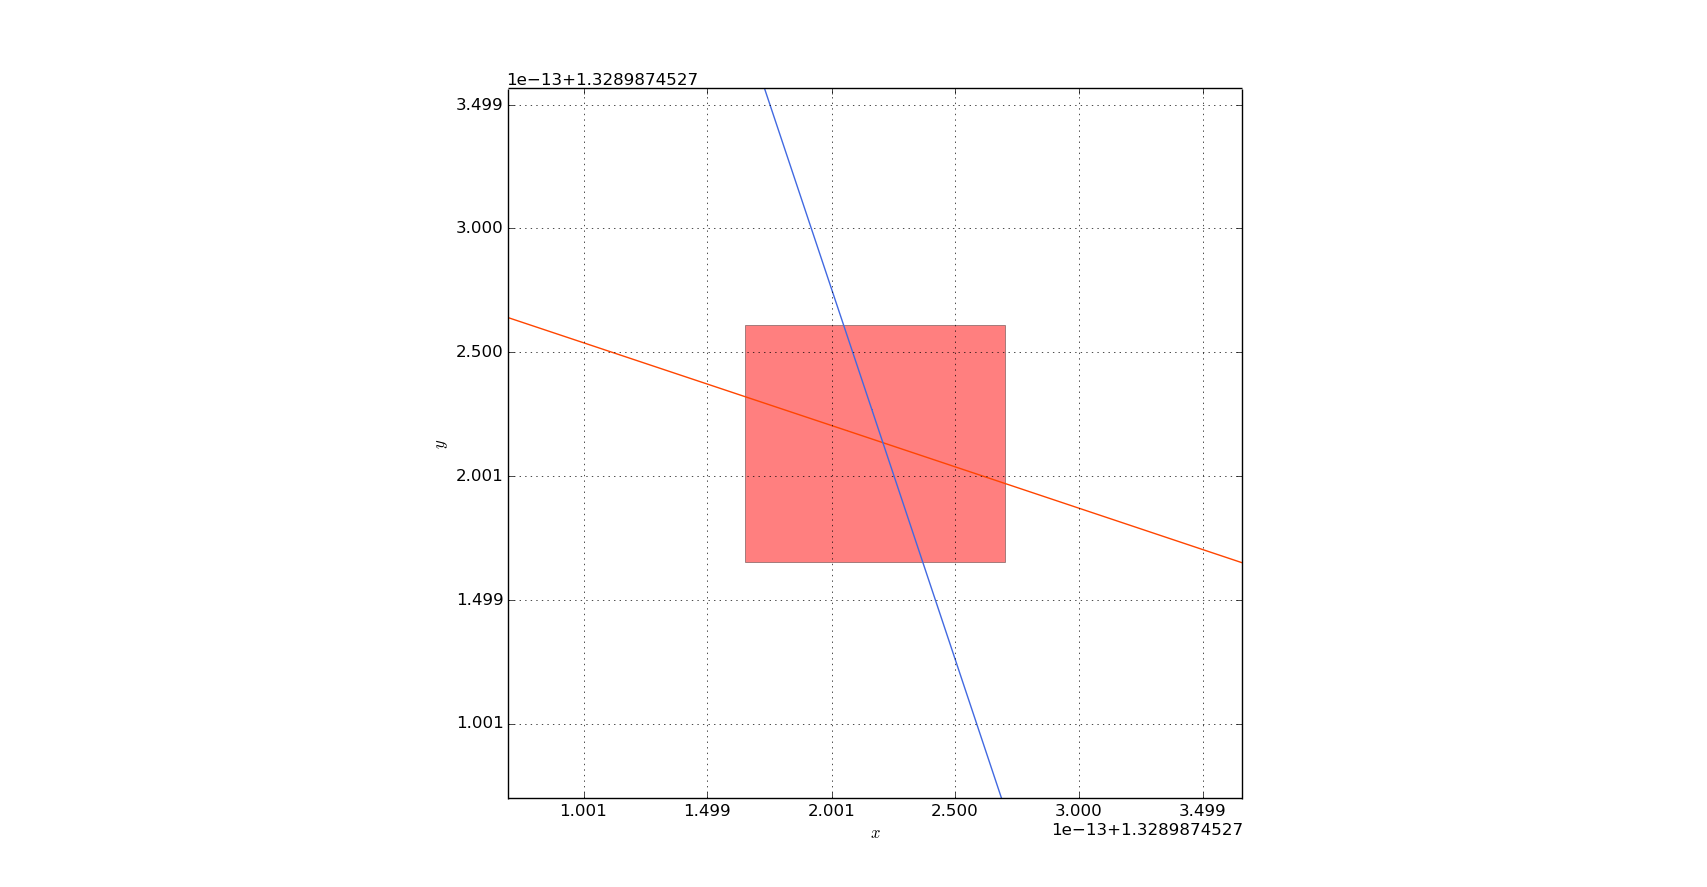
\includegraphics[scale=0.4]{cruce5}
\caption{Cruce de $W^{u},W^{s}$ encontrado con el intervalo e }
\label{cruce5}
\end{figure}

\begin{figure}[H]
\centering
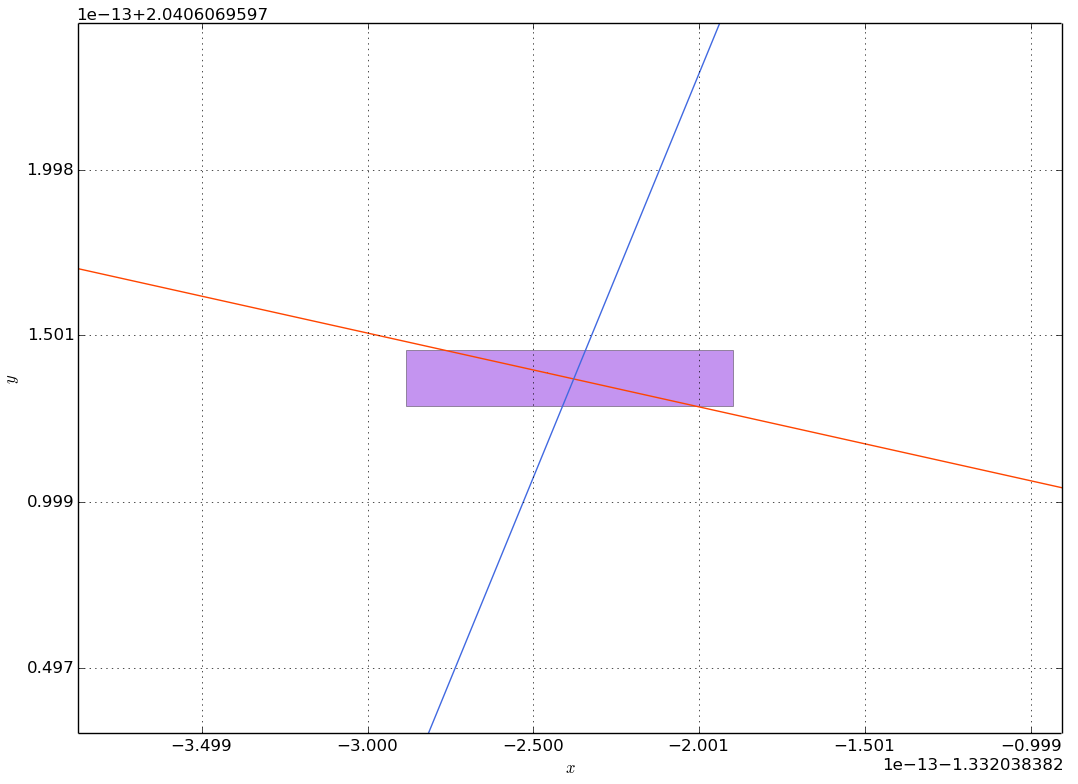
\includegraphics[scale=0.4]{cruce6}
\caption{Cruce de $W^{u},W^{s}$ encontrado con el intervalo f }
\label{cruce6}
\end{figure}

\begin{figure}[H]
\centering
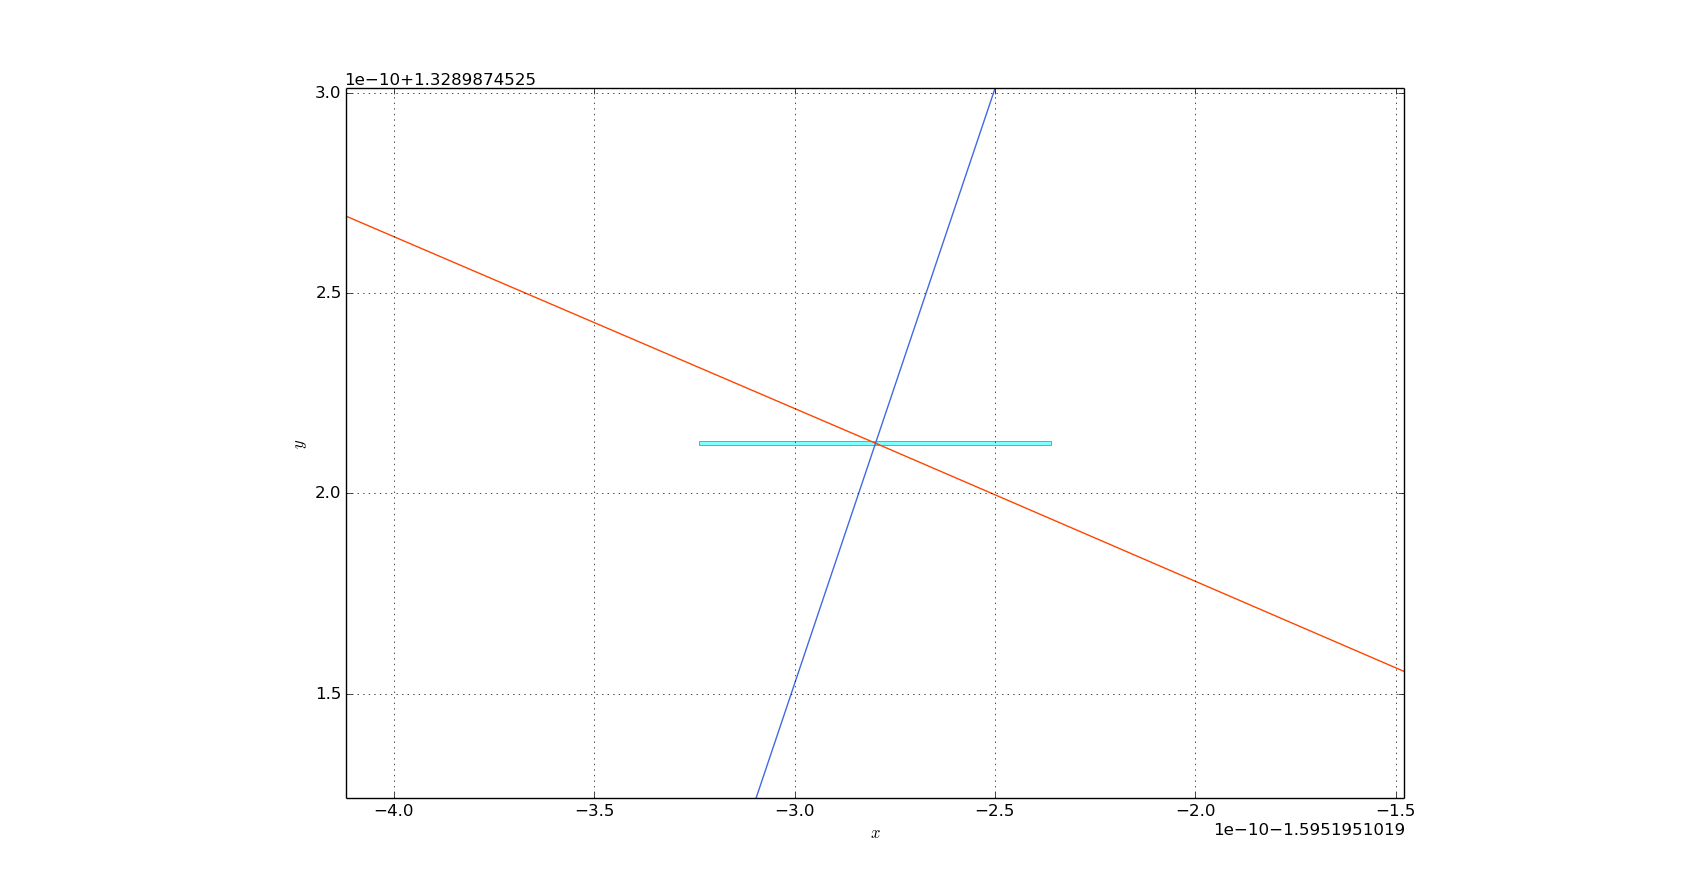
\includegraphics[scale=0.4]{cruce7}
\caption{Cruce de $W^{u},W^{s}$ encontrado con el intervalo g }
\label{cruce7}
\end{figure}

\begin{figure}[H]
\centering
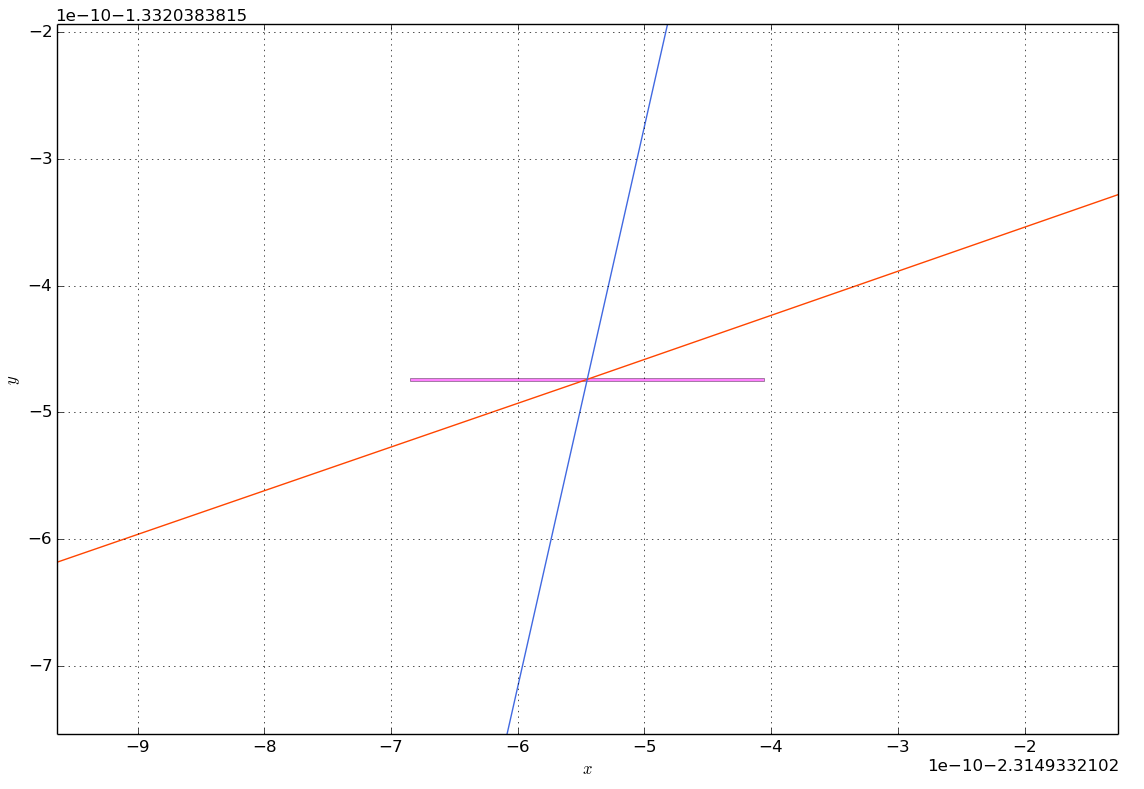
\includegraphics[scale=0.4]{cruce8}
\caption{Cruce de $W^{u},W^{s}$ encontrado con el intervalo h }
\label{cruce8}
\end{figure}


La zona rectangular sombreada en cada gráfica representa el producto cruz de los intervalos donde se encuentra la solución. Podemos observar que de hecho cada zona contiene el cruce de las variedades. Garantizando así que en el intervalo propuesto hay un cruce de variedades. Este tipo de resultados son útiles para hablar sobre caos. Hay que aclarar que los intervalos en los que se encuentra la intersección son intervalos en términos de los parámetros, no de las coordenadas del espacio fase, sin embargo conociendo cómo se mapean los intervalos en cada variedad podemos definir un nuevo intervalo en el espacio fase. \\


Para complementar todo este análisis se puede obtener una gráfica de las superficies que forman las variedades al cambiar el parámetro del mapeo lo que nos da una idea de como se ven las superficies y además de como se comportan las intersecciones. Las gráficas correspondientes a esto se encuentran en el sitio \textbf{LIGA}.
\subsection{Mapeo exponencial}
Además se analizaron los cruces en las variedades , usando como en los casos anteriores el mapeo inverso \ref{jungI}. Este mapeo representa un mayor reto en cuanto al orden del polinomio, la presencia de la exponencial hace que la parametrización sea sensible al orden del polinomio. Para el siguiente ejemplo se necesitó un polinomio de orden 86, en el cual se podía observar un comportamiento interesante, y se calcularon los cruces de las variedades como en los otros casos. 



\begin{figure}[H]
\centering
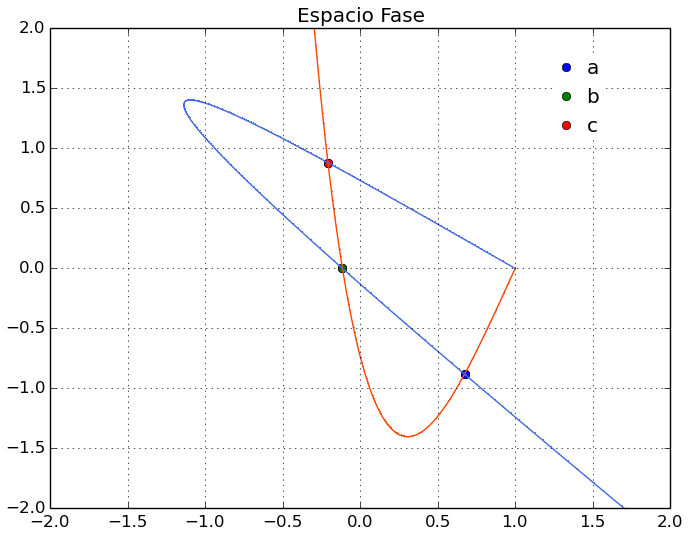
\includegraphics[scale=0.5]{cruces_jung1}
\caption{Intersecciones en el mapeo exponencial con $a=5.7$}
\label{jung_cortes}
\end{figure}
\begin{itemize}
\item[a)] Root$([-0.985068, -0.985067] \times [5.99488, 5.99489]$, :unique)
\item[b)] Root$([-3.46215, -3.46214] \times [5.49229, 5.4923]$, :unique)
\item[c)] Root$([-3.77896, -3.77895] \times [1.56269, 1.5627]$, :unique)
\end{itemize}
Tomando los cruces a escala del intervalo resultan las siguientes gráficas.

\begin{figure}[H]
\centering
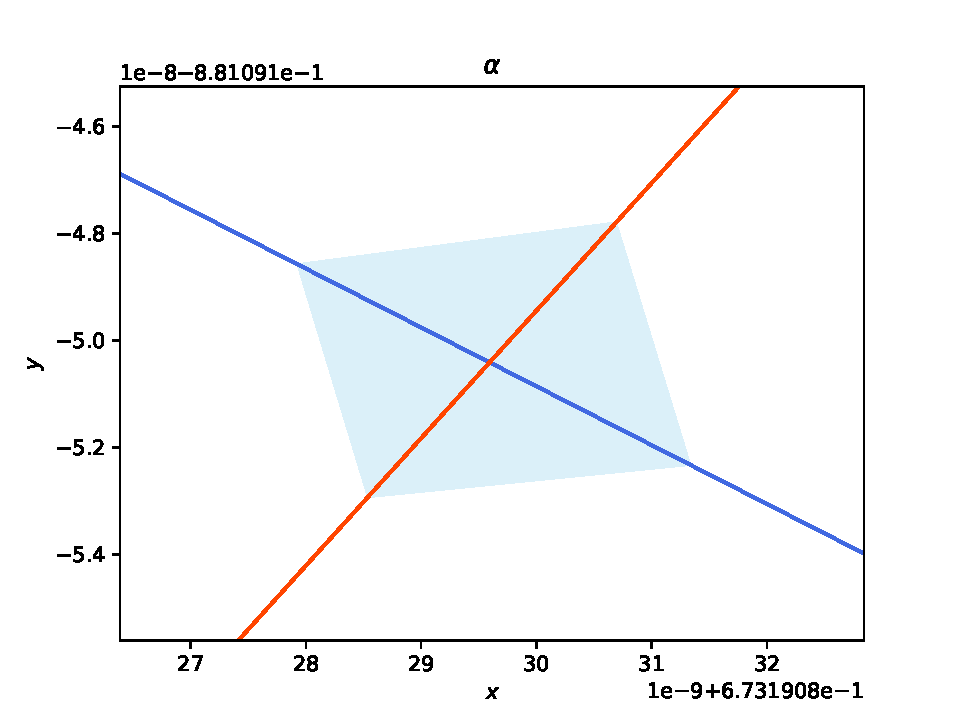
\includegraphics[scale=0.4]{cruce_a}
\caption{Intersección en el intervalo a}
\label{jung_corte1}
\end{figure}


\begin{figure}[H]
\centering
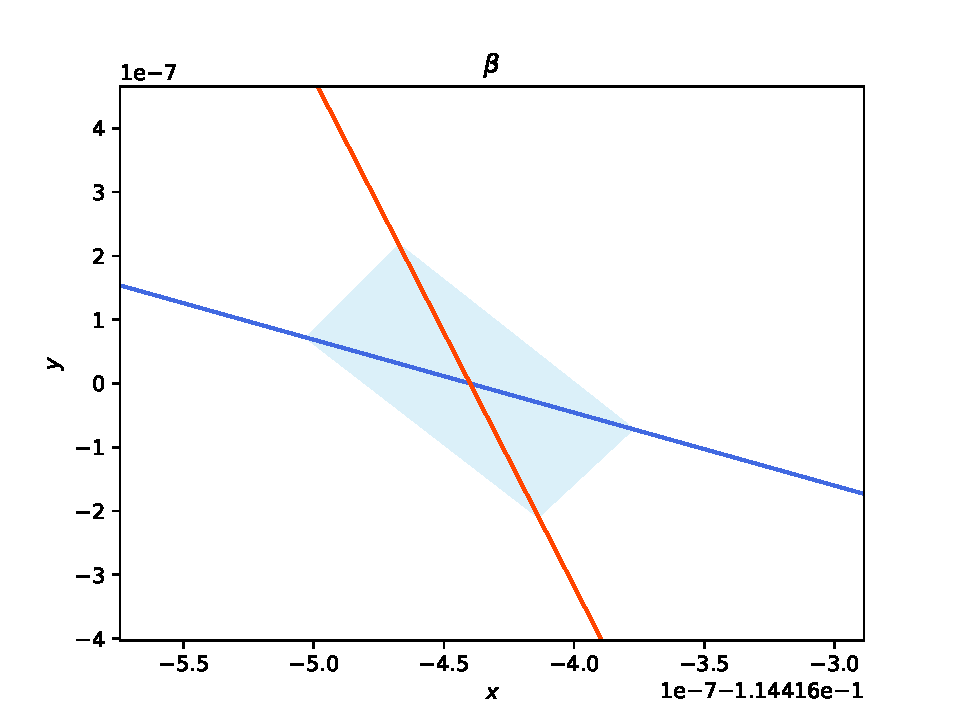
\includegraphics[scale=0.4]{cruce_b}
\caption{Intersección en el intervalo b}
\label{jung_corte2}
\end{figure}


\begin{figure}[H]
\centering
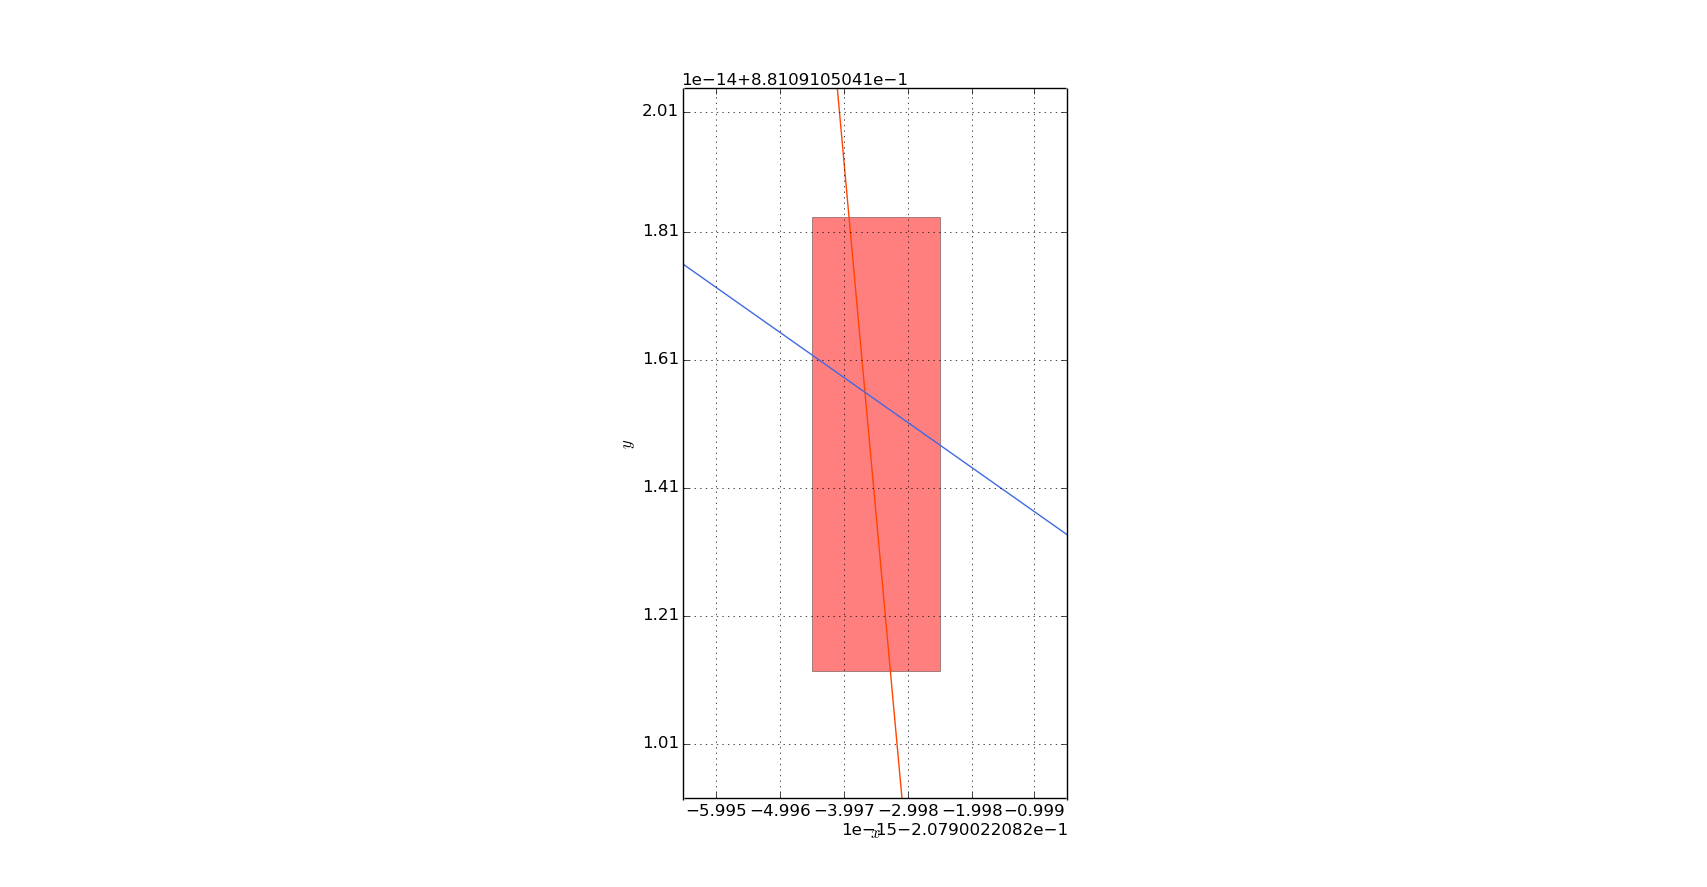
\includegraphics[scale=0.4]{cruce_c}
\caption{Intersección en el intervalo c}
\label{jung_corte3}
\end{figure}



